% Candidate extraction from a resolution log; this is not kernel replay.
% Build: pdflatex resolution_evidence.tex
\documentclass[tikz,border=3pt]{standalone}
\usepackage{lmodern,amsmath,amssymb}
\usetikzlibrary{arrows.meta,calc}
\begin{document}
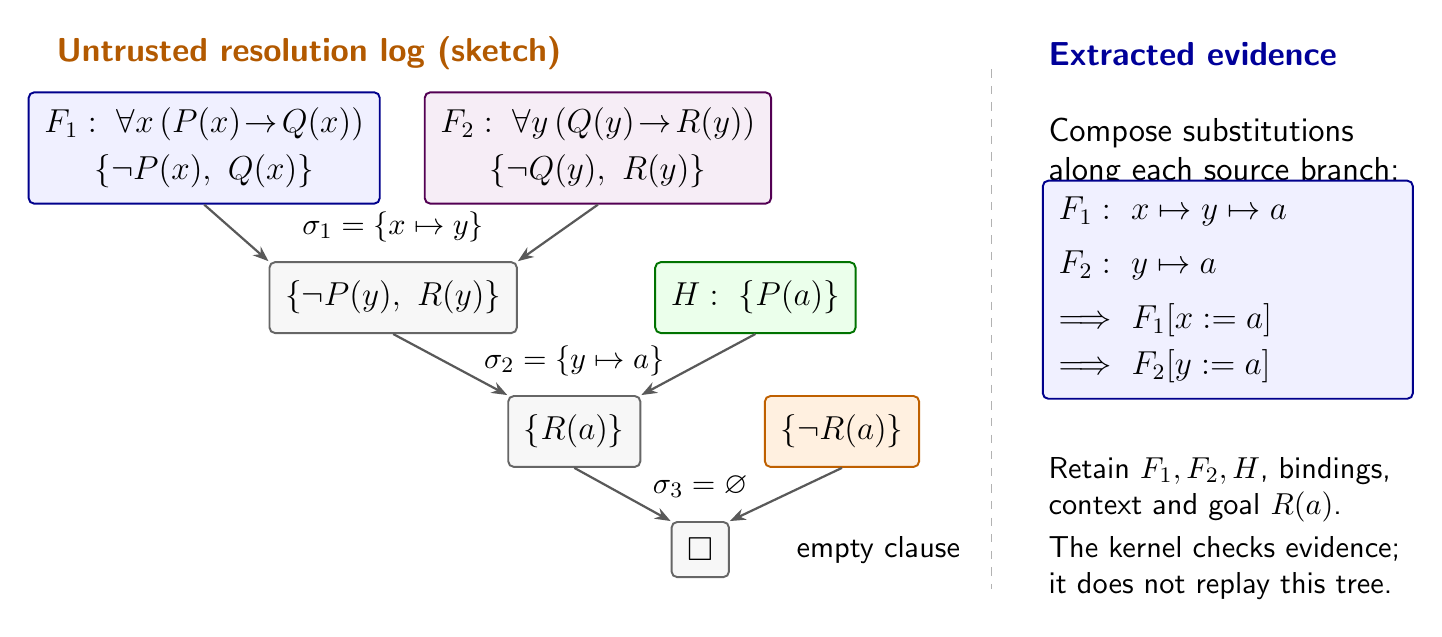
\begin{tikzpicture}[
  font=\sffamily\fontsize{12}{14}\selectfont,
  clause/.style={draw=blue!55!black,fill=blue!6,rounded corners=2pt,
    line width=.7pt,align=center,inner sep=2mm,minimum height=9mm},
  fact/.style={clause,draw=green!45!black,fill=green!8},
  neggoal/.style={clause,draw=orange!75!black,fill=orange!12},
  derived/.style={clause,draw=black!60,fill=black!3},
  flow/.style={-{Stealth[length=2mm]},line width=.8pt,black!65},
  subst/.style={fill=white,inner sep=1pt,font=\sffamily\fontsize{11}{13}\selectfont},
  heading/.style={font=\sffamily\bfseries\fontsize{13}{15}\selectfont,anchor=west},
]
\node[heading,text=orange!70!black] at (0,12mm) {Untrusted resolution log (sketch)};
\node[clause] (f1) at (20mm,0) {$F_1:\ \forall x\,(P(x)\!\to\!Q(x))$\\[1mm]$\{\neg P(x),\ Q(x)\}$};
\node[clause,draw=violet!65!black,fill=violet!7] (f2) at (70mm,0)
  {$F_2:\ \forall y\,(Q(y)\!\to\!R(y))$\\[1mm]$\{\neg Q(y),\ R(y)\}$};
\node[derived] (r1) at (44mm,-19mm) {$\{\neg P(y),\ R(y)\}$};
\draw[flow] (f1.south) -- (r1.north west);
\draw[flow] (f2.south) -- (r1.north east);
\node[subst] at (44mm,-10mm) {$\sigma_1=\{x\mapsto y\}$};
\node[fact] (h) at (90mm,-19mm) {$H:\ \{P(a)\}$};
\node[derived] (r2) at (67mm,-36mm) {$\{R(a)\}$};
\draw[flow] (r1.south) -- (r2.north west);
\draw[flow] (h.south) -- (r2.north east);
\node[subst] at (67mm,-27mm) {$\sigma_2=\{y\mapsto a\}$};
\node[neggoal] (g) at (101mm,-36mm) {$\{\neg R(a)\}$};
\node[derived,minimum height=7mm] (empty) at (83mm,-51mm) {$\square$};
\draw[flow] (r2.south) -- (empty.north west);
\draw[flow] (g.south) -- (empty.north east);
\node[subst] at (83mm,-43mm) {$\sigma_3=\varnothing$};
\node[anchor=west,font=\sffamily\fontsize{11}{13}\selectfont] at (94mm,-51mm) {empty clause};
\draw[black!30,dashed] (120mm,10mm) -- (120mm,-56mm);
\node[heading,text=blue!60!black] at (126mm,12mm) {Extracted evidence};
\node[anchor=north west,align=left] at (126mm,5mm)
  {Compose substitutions\\along each source branch:};
\node[clause,text width=43mm,align=left] at (150mm,-18mm)
  {$F_1:\ x\mapsto y\mapsto a$\\[2mm]
   $F_2:\ y\mapsto a$\\[2mm]
   $\Longrightarrow\ F_1[x:=a]$\\[1mm]
   $\Longrightarrow\ F_2[y:=a]$};
\node[anchor=north west,align=left,font=\sffamily\fontsize{11}{13}\selectfont] at (126mm,-38mm)
  {Retain $F_1,F_2,H$, bindings,\\context and goal $R(a)$.\\[1mm]
   The kernel checks evidence;\\it does not replay this tree.};
\end{tikzpicture}
\end{document}
